\section{Ergebnisse und Diskussion}
\label{sec:discuss}

\subsection{Modellwahl}
\label{ssec:discuss:modelselect}
Unter Anwendung der in Abschnitt \ref{ssec:modellselektion} bzw \ref{ssec:impl:modelwahl} vorgestellten Methode wurde aus einem 149 Prädiktoren umfassenden Maximalmodell das in Tabelle \ref{table:model_parameters} angegebene, 50 Prädiktoren große Modell anhand des kleinsten $C_p$-Wertes von $\m{\approx3.92}$ als optimales Modell ausgewählt.\\
\begin{figure*}[ht]
    \centering
    \begin{tikzpicture}
        \begin{axis}[ 
            ylabel = $N_{origin}$,
            xlabel = $N_{est}$,
            xmin=0, xmax=0.8,
            ymin=0, ymax=0.8,
            legend pos = north west,
            scaled ticks = false,
            width = .5\textwidth,
            ymajorgrids,
            xmajorgrids,
            %height = 8cm,
            cycle list name=black white
        ]
            \addplot +[only marks]
            table[x=origN, y=simN, col sep=comma] {plots/data/correlation_plot_data.csv};
            %\addlegendentry{{\scriptsize Variablität}}
            \begin{scope}[red]
                \draw[red] ({axis cs:0,0}) -- ({axis cs:1,1});
            \end{scope}   
            %\addplot +[ycomb, no marks, dashed] 
            %table[x=x, y expr=0.0105 ,col sep=comma] {plots/data/selectedFeatures.csv};
            
            
        \end{axis}
    \end{tikzpicture}
    \captionof{figure}{Korrelationsplot}
    \label{fig:correlation}
\end{figure*}
Der Wert des Bestimmtheitsmaßes $R^2 = 0.82$ zeigt, dass das gewählte Modell die Varianz in den Daten gut erklären kann. Dies spiegelt auch das in Abbildung \ref{fig:correlation} abgebildete Korrelationsdiagramm wieder, in welchen der wahre Wert auf der x-Achse und der geschätzte Stickstoffmengenanteil auf der y-Achse aufgetragen sind.
Abweichungen sind lediglich im unteren Bereich zwischen $0.0$ und $0.03$ und ab $0.3$ zu beobachten, wo der Stoffmengenanteil des Stickstoffs durch das Modell unterschätzt wird.
Dies lässt dich vermutlich durch die geringe Datendichte in diesen Bereichen erklären.
Insgesamt kann man sagen, dass die bisherigen Untersuchungen auf ausreichend gute Prognosen durch das Modell hindeuten.

\begin{figure}[H]
    \centering
    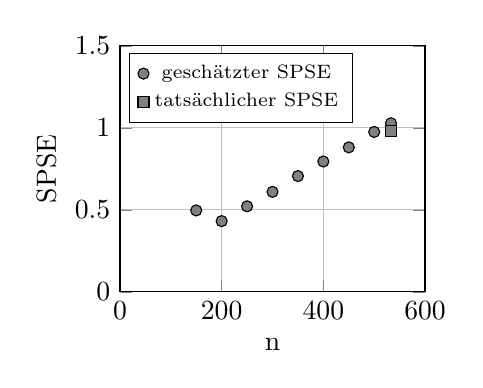
\begin{tikzpicture}
        \begin{axis}[ 
            ylabel = SPSE,
            xlabel = n,
            xmin=0, xmax=600,
            ymin=0, ymax=1.5,
            legend pos = north west,
            scaled ticks = false,
            width = .45\textwidth,
            ymajorgrids,
            xmajorgrids,
            %height = 8cm,
            cycle list name=black white
        ]
            \addplot +[only marks]
            coordinates {
                (150,0.4964226)
                (200,0.4312206)
                (250,0.5213190)
                (300,0.6097658)
                (350,0.7058959)
                (400,0.7947748)
                (450,0.8807918)
                (500,0.9750933)
                (533,1.0280917)
            };
            \addlegendentry{{\scriptsize geschätzter SPSE}}
            
            \addplot +[only marks]
            coordinates {
                (533,0.9813258)
            };
            \addlegendentry{{\scriptsize tatsächlicher SPSE}}
        \end{axis}
    \end{tikzpicture}
    \captionof{figure}{geschätzer sowie tatsächlicher SPSE in Abhängigkeit der Stichprobengröße}
    \label{fig:spse}
\end{figure}